\documentclass[times, 10pt,twocolumn]{article}

\usepackage{sose2011}
\usepackage{times}
\usepackage{color}
\usepackage[pdftex]{graphicx}

\graphicspath{{./images/}}
\DeclareGraphicsExtensions{.pdf,.jpeg,.png,.jpg}

% correct bad hyphenation here
\hyphenation{op-tical net-works semi-conduc-tor}
\pagestyle{empty}

\begin{document}

\title{Managed Control of Composite Cloud Systems}

\author{
        \textbf{Christopher C. Lamb}\hspace*{0.1in}
        \textbf{Pramod A. Jamkhedkar}\hspace*{0.1in}
        \textbf{Gregory L. Heileman}\hspace*{0.1in}
        \textbf{Chaouki T. Abdullah}\\
        Department of Electrical and Computer Engineering \\
        University of New Mexico \\
        \small{\{cclamb, pramod54, heileman, chaouki\}@ece.unm.edu}
}

\maketitle
\thispagestyle{empty}

\begin{abstract}
Cloud providers have just begun to provide primitive functionality enabling users to configure and easily provision resources, primarily in the infrastructure as a service domain.  In order to effectively manage cloud resources in an automated fashion, systems must automate quality-of-service (QoS) metric measurement as a part of a larger usage management strategy.  Collected metrics can then be used within control loops to manage and provision cloud resources.  This basic approach can be scaled to monitor the use of system artifacts as well as simple QoS parameters, and can also address the needs of large systems spanning the boundaries of single service providers though the problem seems to moving toward intractability.
\end{abstract}

{
\setlength{\parindent}{0mm}
\textbf{Keywords:} Usage Management, Cloud Computing, System of Systems.
}

\section{Introduction}
Cloud computing services as a computational paradigm are more market oriented than previous attempts at commodity computing.  Furthermore, they are in many cases designed to be composed into larger, more powerful customer facing systems.  These kinds of aggregate systems fit neatly into one of the more commonly used definitions of a system of systems as well \cite{Sose:SageCuppan:2001}, \cite{Sose:Web:Defns}.  With so much data in the hands of different providers in an aggregate system, system developers and users are hard-pressed to effectively monitor and control the use of sensitive content by various composite systems.  Some of this information can be contained in Service Level Agreements (SLAs), but they have thus far been focused on quality-of-service (QoS) metrics rather than addressing issues like data flow or physical application residency.  For the most part SLAs are simply not sufficient for addressing usage management concerns \cite{WSA}, \cite{WSLA}, \cite{WSP}, \cite{PaRaSh:09}.

Effective usage management monitoring coupled with feedback processing creates an event loop suitable for applying control theoretic concepts to cloud infrastructures.

Usage policies specified at a fine-grained level provides cloud service users with more reliability of the use of their data within cloud-centric systems.  For example, data routing, caching, or hosting can be a sensitive issue for some systems in that specific users may want to restrict the countries that can access that data.  The ability to specify and control where specifically that data travels and resides gives those kinds of sensitive users confidence to use cloud-centric computing resources.  Furthermore, this kind of control will also facilitate cost profiles for services that more closely match demand, giving providers better control over their infrastructure and additional areas for product differentiation.

Herein, we will elaborate the idea of applying usage management to single and distributed cloud systems.  In this brief analysis, we will touch on the application of common system design principles and standards \cite{BlCl:01}, \cite{Cl:88}, \cite{ClWrSoBr:02}, application of usage control concepts \cite{PaSa:04}, control theory as applied to computing systems \cite{ctrl:Zhu:2009:CTB:1496909.1496922}, \cite{ctrl:ariba-GL:2009}, \cite{ctrl:wang-cgswrzh:2009}, \cite{ctrl:kjaer-kr:2009}, \cite{ctrl:abdelwahed-bsk:2009}, \cite{ctrl:hellerstein-sw:2009}, and interoperability~\cite{JaHe:04}, \cite{HeJa:05}, \cite{KoLaMaMi:04}, \cite{coral}, \cite{marlin}.  We will apply these ideas toward a controllable feedback-enabled system suitable for cloud system control.

In Section~\ref{sec:single} this paper first addresses how to create a controllable system with feedback suitable for system evaluation from the perspective of a single provider. Here, we will address the constraints and advantages of such an approach and how providers could begin to offer these kinds of services.  In this first example, we will focus on QoS data specifically.  Next in Section~\ref{sec:singleUm} we will extend our single provider system to provide control over attributes more specific to the usage management domain, with examples and associated analysis.  Finally in Section~\ref{sec:multiple} we extend this single provider model to a system deployed to multiple cloud providers in a realistic system-of-systems scenario.

\subsection{Previous Work}
Cloud computing is emerging as the future of utility systems hosting for consumer-facing applications.  In these kinds of systems, components, applications, and hardware are provided as utilities over the Internet with associated pricing schemes pegged by system demand.  Users accept specific QoS guidelines that providers use to provision and eventually allocate resources. These guidelines become the basis over which providers charge for services.

Over the past few years multiple service-based paradigms like web services, cluster computing and grid computing have contributed to the development of what we now call cloud computing~\cite{Bu:09}. Cloud computing distinctly differentiates itself from other service-based computing paradigms via a collective set of distinguishing characteristics:  market orientation, virtualization, dynamic provisioning of resources, and service composition via multiple service providers~\cite{BuYeVeBrBr:09}. This implies that in cloud computing, a cloud-service consumer's data and applications reside inside that cloud provider's infrastructure for a finite amount of time.  Partitions of this data can in fact be handled by multiple cloud services, and these partitions may be stored, processed and routed through geographically distributed cloud infrastructures. These activities occur within a cloud, giving the cloud consumer an impression of a single virtual system.  These operational characteristics of cloud computing can raise concerns regarding the manner in which cloud consumer's data and applications are managed within a given cloud. Unlike other computing paradigms with a specific computing task focus, cloud systems enable cloud consumers to host entire applications on the cloud (i.e. Software as a Service) or to compose services from different providers to build a single system. As consumers aggressively start exploiting these advantages to transition IT services to external utility computing systems, the manner in which data and applications are handled within those systems by various cloud services will become a matter of serious concern.

A growing body of research has begun to appear over the past two years applying control theory to tuning computer systems.  These range from controlling network infrastructure \cite{ctrl:ariba-GL:2009} to controlling virtualized infrastructure and specific computer systems \cite{ctrl:wang-cgswrzh:2009}, \cite{ctrl:kjaer-kr:2009} to exploring feedforward solutions based on predictive modeling \cite{ctrl:abdelwahed-bsk:2009}.  Significant open questions remain to research within this field \cite{ctrl:Zhu:2009:CTB:1496909.1496922}, \cite{ctrl:hellerstein-sw:2009}.

\section{Single Provider Feedback System}\label{sec:single}
Controllable cloud systems enable providers to supply more closely targeted, cost effective services while at the same time providing service consumers with the confidence that the data and other artifacts their systems use are protected.  With that as our eventual goal, we first begin with a simple system managing currently accepted QoS parameters - system attributes like bandwidth, system memory allocation, and the like.  Specifically, we intend to provide the ability to monitor and control a virtual system hosted on a cloud infrastructure so that response time for a hosted application falls within a specific range of accepted parameters.

In order to manipulate a system to meet a preselected threshold of performance metrics, we must have access to measurement information with respect to factors affecting those metrics and we need to be able to adjust system performance in response to those measurements.  An excellent example is system response time measured at the edge of the cloud provider's infrastructure as the metric we wish to control.  We could very well adjust system performance to meet that metric by manipulating the number of processing nodes, bandwidth available to those nodes, and node RAM allocations.

We have identified the attributes we wish to control.  This leads us to a group of requirements we can use to assemble a logical system architecture.  Requirements we know we need to address include:

\begin{itemize}
\item \textit{Performance:} We will be adjusting a system within specific soft real-time frames.  Ergo, we need to be able to collect feedback measurements, process those measurements, and make decisions about how to respond to those measurements quickly in order to avoid falling out of compliance with any performance parameters to which we must adhere.
\item \textit{Accessibility:} In order to control component systems, we must be able to access those systems.  In order to do so within time constraints, we must be able to access those systems electronically as well; physical access requirements simply will not scale into this performance domain.
\item \textit{Controllability:} We must be able to access the appropriate control primitives on the systems we need to tune.  This will include accessing compute node generation and termination capabilities.  It would help if we could access node performance information and tune those nodes as well, though this is not required; we can emulate this by terminating nodes in one configuration and creating nodes with another to more adequately address performance needs.
\end{itemize}

These system attributes lead us to a system architecture that is beginning to look like a traditional feedback-centric controllable system.

\begin{figure}[!t]
\centering
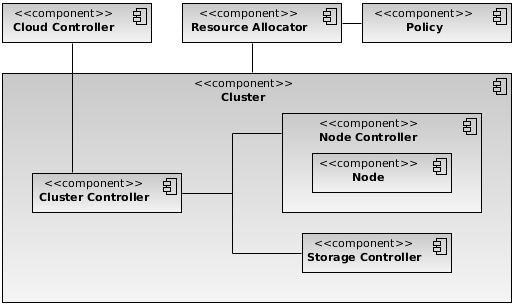
\includegraphics[width=3in]{Single-QoS}
\caption{Single Cloud Provider, Quality of Service.}
\label{fig:single-qos}
\end{figure}

The system shown in Figure \ref{fig:single-qos} seven primary components.  These components work together to provide cloud services to consumers in a hypothetical infrastructure-as-a-service scenario.  This particular view addresses logical, functional components of this kind of a system rather than specific technologies used in an implementation, although some components are loosely modeled on popular open-source cloud environments (i.e. Eucalyptus).

Essentially, we have a cloud controller element that initiates provisioning of compute nodes within a given cluster. The cluster itself is managed by a cluster controller, which in turn controls storage controllers, node controllers, and by extension, nodes.  The nodes and node controllers themselves are monitored by a Resource Allocator which refers to a set of QoS requirements.

\begin{itemize}
\item \textit{Cloud Controller:} Provides an initial interface to administrative users to control the cloud.
\item \textit{Cluster Controller:} Managed by the cloud controller, the cluster controller manages the resources of a single cluster. A given cloud may contain multiple clusters.
\item \textit{Storage Controller:} Provides storage of system images and for other general storage needs.  This controller component is highly I/O sensitive.
\item \textit{Node Controller:} Responsible for allocating, delivering, and managing individual compute nodes upon which client software runs.
\item \textit{Node:} The compute node delivering services to end users and managed by the cluster's control infrastructure.  This is the primary computational resource accessed by users accessing managed cloud resources.
\item \textit{Policy:} Quality of service terms the cloud provider has agreed to honor for the cloud customer with respect to system delivery, provisioning, and overall performance.
\item \textit{Resource Allocator:} The component responsible for real-time tuning of the cloud system to maintain defined quality of service.
\end{itemize}

Operationally, the initial commands required to initialize the cloud are delivered from the \textit{Cloud Controller} to the \textit{Cluster Controller}, who then propagates another, related set of commands provisioning an initial set of resources from the \textit{Node Controllers} and the \textit{Storage Controllers}.  At this point, the initial system has been configured and is running, serving hosted software to its customer base.

Once the system is running, state data describing the performance metrics of interest is dispatched from \textit{Nodes} on the \textit{Node Controllers}, the \textit{Node Controllers} themselves, and the \textit{Storage Controller} to the \textit{Resource Allocator}.  The \textit{Resource Allocator} then processes this new event data in the context of the defined \textit{QoS} parameters.  This processing, in this model, is likely to be simple processing over the current event package or perhaps the current and the otherwise most recent event package.  This evaluation is very performance sensitive; we need to process the state of the current system quickly and adjust resource allocation accordingly.  Because of this soft real-time requirement, we do not have the luxury of spending significant time reviewing trending or providing sophisticated analysis over delivered event information.  Note that extension of this system into the feedforward domain would allow this kind of more robust system management, allowing us to employ more complex and powerful machine learning or neural systems to predict system needs.

Finally, if needed the \textit{Resource Allocator} will dispatch messages to the \textit{Cluster Controller}, \textit{Node Controller}, \textit{Nodes}, and \textit{Storage Controller} adjusting system profiles to ensure they remain within acceptable performance ranges.

\begin{figure}[!t]
\centering
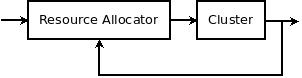
\includegraphics[width=3in]{feedback}
\caption{Control System Perspective.}
\label{fig:feedback}
\end{figure}

As shown in Figure \ref{fig:feedback}, we have an initial reference input reflecting the control parameters outlined by the \textit{Policy}.  The \textit{Resource Allocator} then processes both the reference input as well as system feedback metrics, providing control stimulus to the cloud cluster as output.

This control infrastructure as it has strict timing requirements with respect to event collection, analysis, and control, likely needs to be hosted in close physical proximity to the controlled systems.  Otherwise, the systems themselves can be located just about anywhere accessible to the Internet.  These logical components are not necessarily all hosted on physically distinct systems either, though generally at least the \textit{Storage Controller} and the \textit{Node Controller} are as they have remarkably different requirements with respect to processing power and I/O throughput.

Clearly, both the cloud service consumer and providers are impacted by this kind of infrastructure.  Consumers have systems performing within required performance bounds while providers are no longer required to maintain as strict administrative over-watch of managed systems.  This kind of systems may also impact system developers, as this kind of dynamic node control and allocation imparts new requirements with respect to intra-system data handing and processing.  Generally however, accepted service development guidelines with respect to statelessness and allowing running processes to terminate prior to node shutdown will alleviate these issues.

When implemented, this kind of system will provide dynamic runtime control of cloud systems enhancing provider and customer confidence in the hosted infrastructure's performance potential.  This can also be extended into the usage management realm with more specific requirements with respect to how customer artifacts are managed, not just delivered.

\section{Single Provider Feedback System with Usage Management}\label{sec:singleUm}
Now that we have developed a cloud system capable of fairly granular control via a feedback control loop using QoS parameters, we will next incorporate specific usage management parameters.  In order to provide control over customer data artifacts in a cloud environment, we will adopt the system developed in Section \ref{sec:single}.  Our usage managment control system must fit within the functional confines of the QoS system from Section \ref{sec:single} while extending the QoS functionality to artifacts not generally controlled via traditional QoS metrics.  For these purposes, a good example of an artifact not generally controlled via QoS parameters could be streaming network data.  While bandwidth throttling is clearly in the QoS domain, more specific uses of that data stream like caching and routing are not.   

Using a data stream as an example, we recognize some situations we clearly need to be able to control.  In this example, we will limit ourselves to a data stream emitted from a \textit{Node} on a \textit{Node Controller} which is routed to a user as a result of a user request.  Here, we have control over stream creation.  We want to limit the ability to update that data stream, we certainly don't want that stream deleted, and we want to limit who may read that stream.  In fact, we can safely assume in this scenario that update and deletion are operations we want to completely forbid, while we may want to limit stream readability, leading us to the primary extended requirement when adding usage management over a network stream in this case:

\begin{itemize}
\item \textit{Accessibility:} Data streamed through the cloud system must be able to be monitored and the accessibility of that stream needs to be dynamically tunable.  This implies that we need to be able to control routing and caching of all streaming data according to user specified conditions.  This also implies that we need to be able to control exactly which \textit{Node Controllers} are able to spawn which \textit{Nodes}.
\end{itemize}

\begin{figure}[!t]
\centering
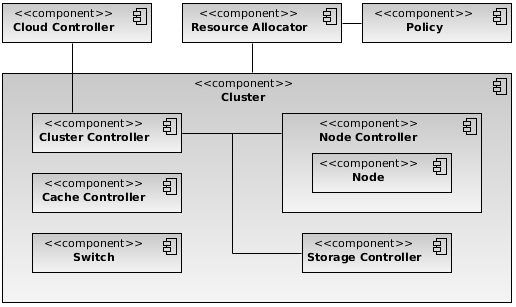
\includegraphics[width=3in]{Single-UM}
\caption{Single Cloud Provider, Usage Management.}
\label{fig:single-um}
\end{figure}

The addition of these attributes and requirements give us the logical system shown in Figure \ref{fig:single-um}.  The new system has new associations and components required to implement the degree of control required to limit the accessibility of the network stream.  We have added \textit{Cache Controllers} and \textit{Switches}, defined as:

\begin{itemize}
\item \textit{Cache Controllers:} Streaming network data, specifically media-centric streams, can and are cached by strategically located cache systems.  In order to control the read access of network data, we must be able to exercise explicit control over any caching systems in our infrastructure.
\item \textit{Switch:} Really any kind of hardware that controls the delivery of network data.  This component includes switches and routers primarily.  In order to control how data is accessed we must be able to control the locations to which it is delivered.
\end{itemize}

We have also added a new relationship to enable control over the \textit{Cloud Controller}.  To ensure that we can control where data is at any given time, we must also be able to control the geographic areas from which data is generated, especially if the virtual compute cloud spans national boundaries.

This again forms a controllable feedback loop, though one that is more complex than the simple QoS case.  The addition of new controllable items and relationships increases the responsibility and complexity of the \textit{Resource Controller} as new logic and capabilities are added to facilitate measurement and control of the larger system.  At this point however, the number of elements of complexity is still increasing linearly, leading us to believe that the problem may in fact still be tractable.

\section{Scaling to Multiple Providers}\label{sec:multiple}
We have briefly examined a single case controlling quality-of-service parameters and a second single case with quality-of-service and usage management parameters.  Moving from the first case to the second did increase the complexity of the problem somewhat, but not significantly.  Now we will expand our scope to multiple cloud providers, as shown in Figure \ref{fig:multiple}.

\begin{figure}[!t]
\centering
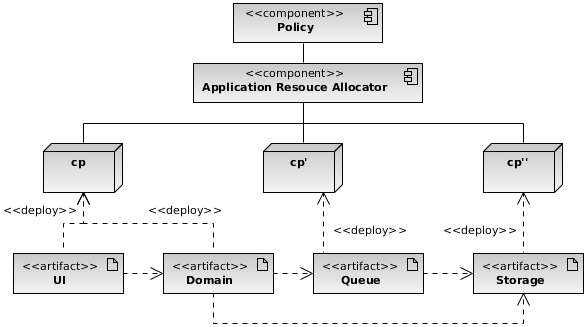
\includegraphics[width=3in]{Multiple}
\caption{Multiple Cloud Providers and hosted application.}
\label{fig:multiple}
\end{figure}

We now have three different cloud providers and various system layers of a sample application mapped to those providers.  The first provider, $ cp $, provides hosting for the \textit{User Interface} and \textit{Domain} layers.  The second provider, $ cp' $, provides queuing services to the application, while the third and final provider, $ cp'' $, provides data storage.  Each cloud provider contains the same elements contained by the providers in the previous sections, including a \textit{Resource Allocator} specific to that cloud provider.

Also, we have a new \textit{Resource Allocator}, an \textit{Application Resource Allocator}.  This new controller is required to provide control over the resources from the application's perspective.  The provider allocation controllers are sufficient for providing control over cloud specific resources from the provider's perspective, but cannot provide the appropriate view into the needs of the application as the application's needs span provider controller domains. As a result, we need a new controller element able to take a holistic, end-to-end view of the applications component systems that can then tune those systems so that application performance is effectively managed.  This effectively gives us a hierarchy of \textit{Resource Allocators}, each dedicated to optimizing a particular combination of resources, ranging from application-centric resources to provider-centric resources or other dependencies.

Here, we have a simple representation of a composite cloud system, a true system-of-systems, in the application implemented on the various cloud providers.  Furthermore, we now have the beginnings of an exponential problem with respect to \textit{application} control.  The complexity of a cloud provider may increase linearly, but the number of possible combinations of tunable parameters is exponential in the number of component systems, hinting at the beginnings of a potentially intractable problem.

\section{Conclusion}
Herein, we introduced the idea of using usage management constructs to manage an infrastructure dedicated to monitoring and tuning distributed and virtualized computing systems.  We began by framing the problem with customary QoS metrics, including a hypothetical system architecture to frame discussion.  We then moved into applying usage management to data entities over the infrastructure, added new requirements and components to the system architecture, and noticed complexity trending.  We finally presented a composite cloud system firmly in the system-of-systems domain addressing additional requirements and possible intractability of application resource allocation and control.

Future planned work in this area involves rigorous analysis of the computational complexity of controlling composite systems.  This will extend into possible heuristics to ameliorate domain complexity as needed.  These systems also require further work addressing usage management of streaming data and ontologies addressing management of typical cloud artifacts.  Once the basic theoretical issues around such control systems are more completely understood, we will develop reference implementations around typical cloud systems illustrating this approach to system monitoring and control.

\bibliographystyle{IEEEtran}
\bibliography{emr,drm,sose,ctrl}

\end{document}


